\section[Desenvolvimento do Projeto]{Desenvolvimento do Projeto}
Nesta seção, são fornecidas informações relativas ao desenvolvimento do projeto, abrangendo a localização do código-fonte e documentação, a arquitetura e as tecnologias utilizadas, bem como os protótipos de tela desenvolvidos. Além disso, são apresentados os artefatos desenvolvidos ao longo do semestre em que o projeto foi realizado. 

\subsection{Repositório do Código Fonte do Projeto}
  Seguem os repositórios do código fonte, eles foram divididos entre front-end e
back-end, utilizando de scripts com um Linter para garantir que o código
permanecesse formatado.

Além disso foram utilizados padrões de commit, no back-end era feat/USnº/nome, já no front era feat/pagina/função.

Front-end:

https://tools.ages.pucrs.br/plataforma-onboarding-para-novoscolaboradores/decola-frontend

Back-end:

https://tools.ages.pucrs.br/plataforma-onboarding-para-novoscolaboradores/decola-api

\subsection{Banco de Dados Utilizado}
  O banco de dados escolhido foi o PostgreSQL, um banco de dados da categoria
relacional, tendo em vista a facilidade e robustez que este tipo de banco oferece, ainda
mais levando em conta que o esquema a ser implementado teria diversas entidades,
tabelas e relações.
Além disso foi usado um mapeador, chamado TypeORM para facilitar a
implementação das funções do banco de dados.

https://tools.ages.pucrs.br/plataforma-onboarding-para-novos-colaboradores/decola-wiki/-/wikis/database
  \begin{figure}[H]
    \centering
    \small
    \caption{Modelagem do Banco de Dados - Decola}
    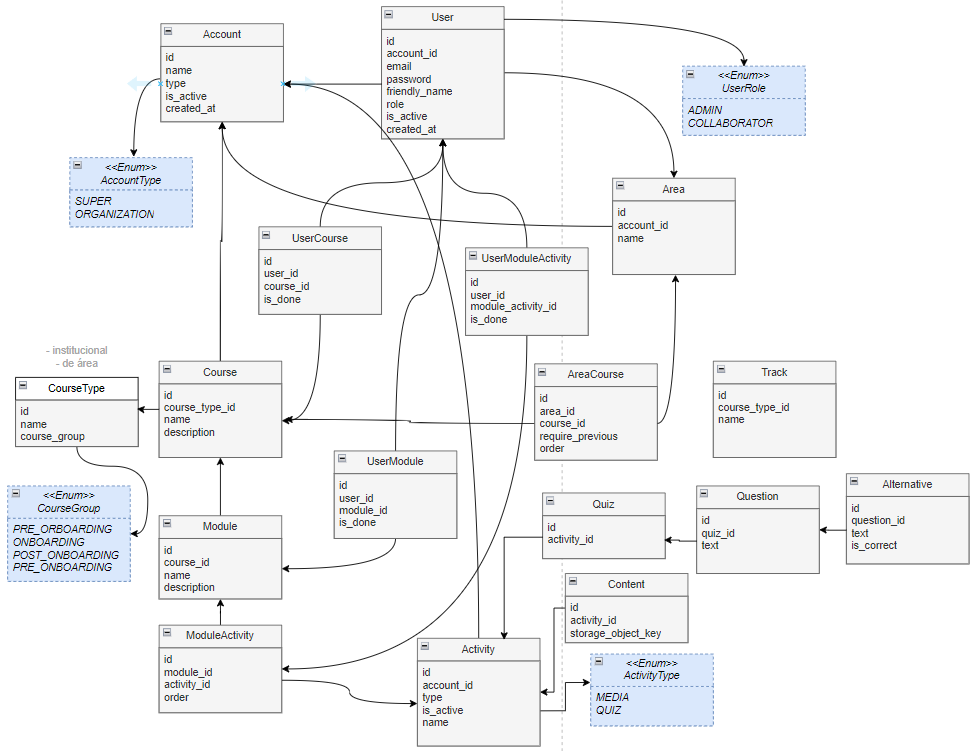
\includegraphics[width=1\linewidth]{conteudo//2 - ages I//conteudo//figures/decola-database.png}
    Fonte: Wiki do Projeto
    \label{fig:database-decola}
\end{figure}

\subsection{Arquitetura Utilizada}
  O modelo de arquitetura escolhido foi o MVC, onde o usuário interage com a
parte de view, o banco de dados interage com o model e o controller integra as duas
anteriores.

    Também faz parte da arquitetura o uso do padrão aberto de segurança JWT, que provê mais segurança para aplicativos e sistemas, através de sistemas de autenticação e autorização, garantindo que apenas usuários autorizados acessem o site.

    \begin{figure}[H]
        \centering
        \small
        \caption{Representação MVC - Decola}
        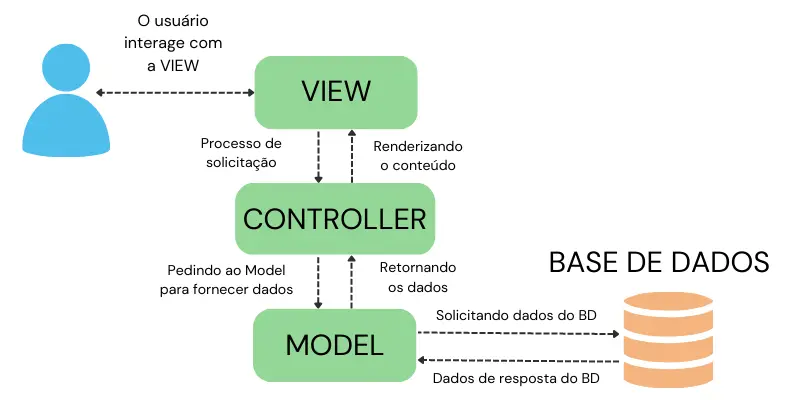
\includegraphics[width=1\linewidth]{conteudo//2 - ages I//conteudo//figures/decola-mvc.jpg}
        Fonte: Wiki do Projeto
        \label{fig:mvc-decola}
\end{figure}

    \begin{figure}[H]
        \centering
        \small
        \caption{Arquitetura Frontend - Decola}
        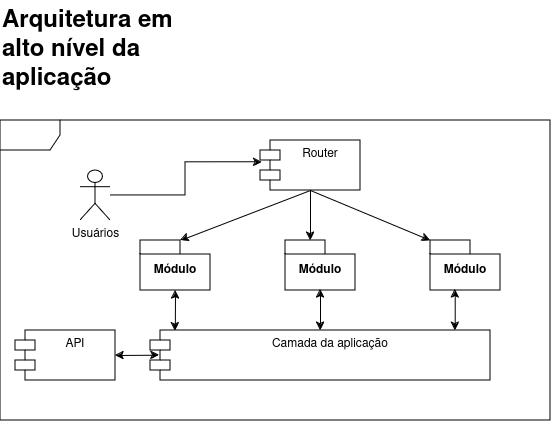
\includegraphics[width=1\linewidth]{conteudo//2 - ages I//conteudo//figures/decola-front-arch.png}
        Fonte: Wiki do Projeto
        \label{fig:arch-front-decola}
\end{figure}

    \begin{figure}[H]
        \centering
        \small
        \caption{Fluxo de autenticação com JWT - Decola}
        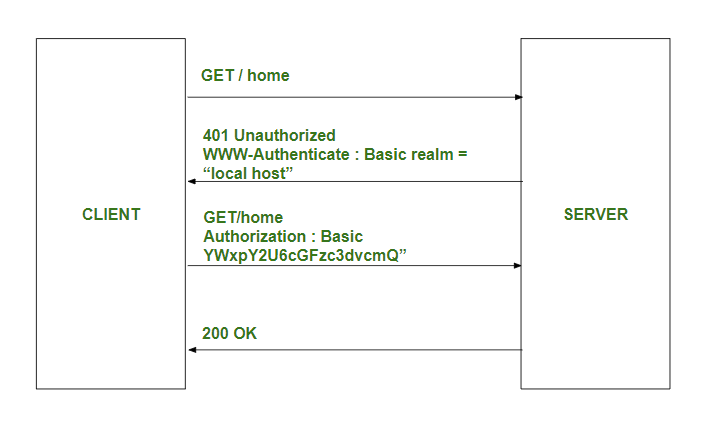
\includegraphics[width=1\linewidth]{conteudo//2 - ages I//conteudo//figures/decola-jwt-auth.png}
        Fonte: Wiki do Projeto
        \label{fig:jwt-decola}
\end{figure}

https://tools.ages.pucrs.br/plataforma-onboarding-para-novos-colaboradores/decola-wiki/-/wikis/arquitetura

\subsection{Protótipos das Telas Desenvolvidas}
    Foram desenvolvidas cerca de 20 telas diferentes, todas passando pelo
    processo de prototipação no Figma e com diferentes versões, incluindo protótipos de
    baixa, média e alta fidelidade, além disso foi utilizada componentização no Figma,
    além de padrões de fontes, variáveis de cores e outros recursos. Seguem abaixo os
    protótipos de alta fidelidade.


  \begin{figure}[H]
    \centering
    \small
    \caption{Mockup Home - Decola}
    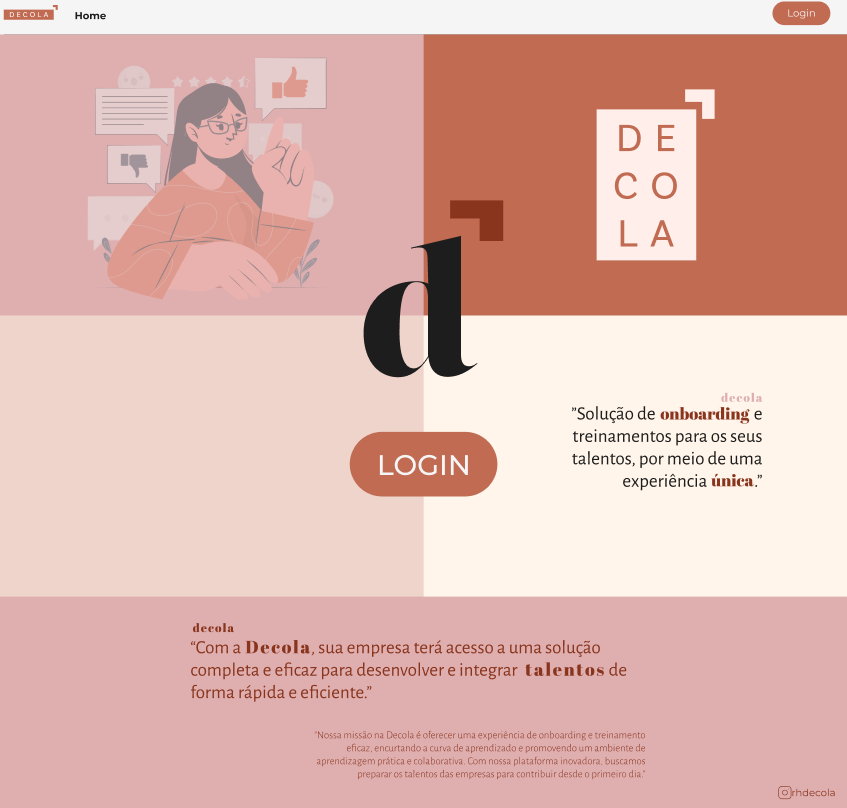
\includegraphics[width=1\linewidth]{conteudo//2 - ages I//conteudo//figures/mockup-decola-home.png}
    Fonte: Wiki do Projeto
    \label{fig:home-mockup-decola}
\end{figure}

    \begin{figure}[H]
        \centering
        \small
        \caption{Mockup Login - Decola}
        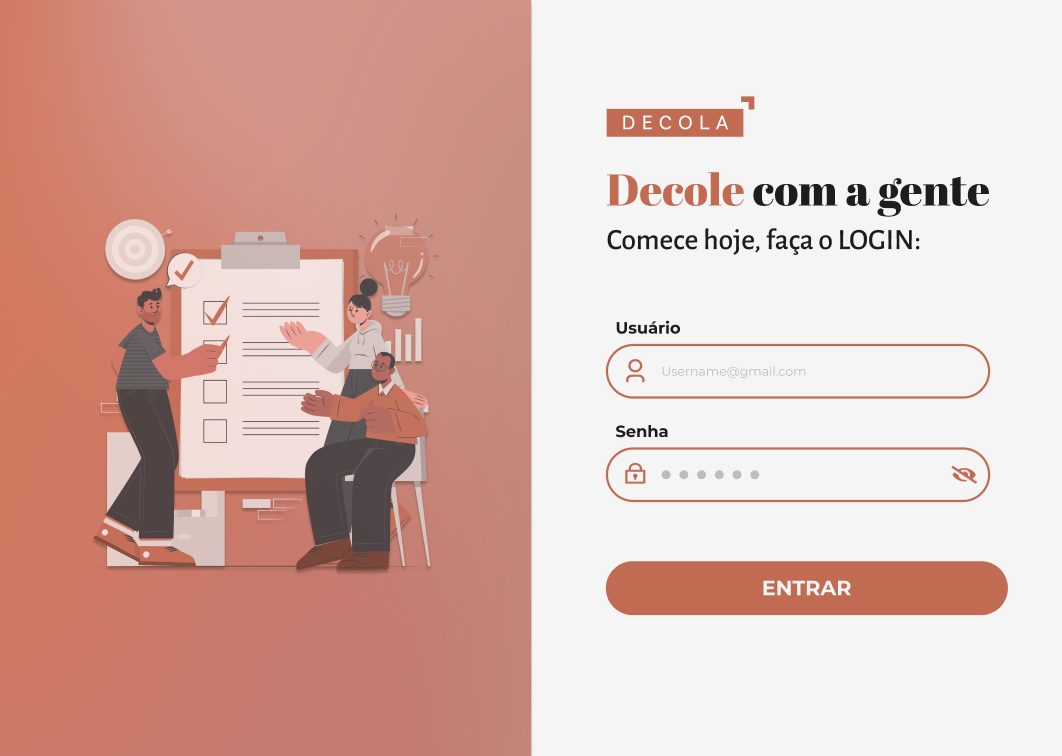
\includegraphics[width=1\linewidth]{conteudo//2 - ages I//conteudo//figures/mockup-decola-login.png}
        Fonte: Wiki do Projeto
        \label{fig:login-mockup-decola}
\end{figure}

    \begin{figure}[H]
        \centering
        \small
        \caption{Mockup Tela Inicial do RH - Decola}
        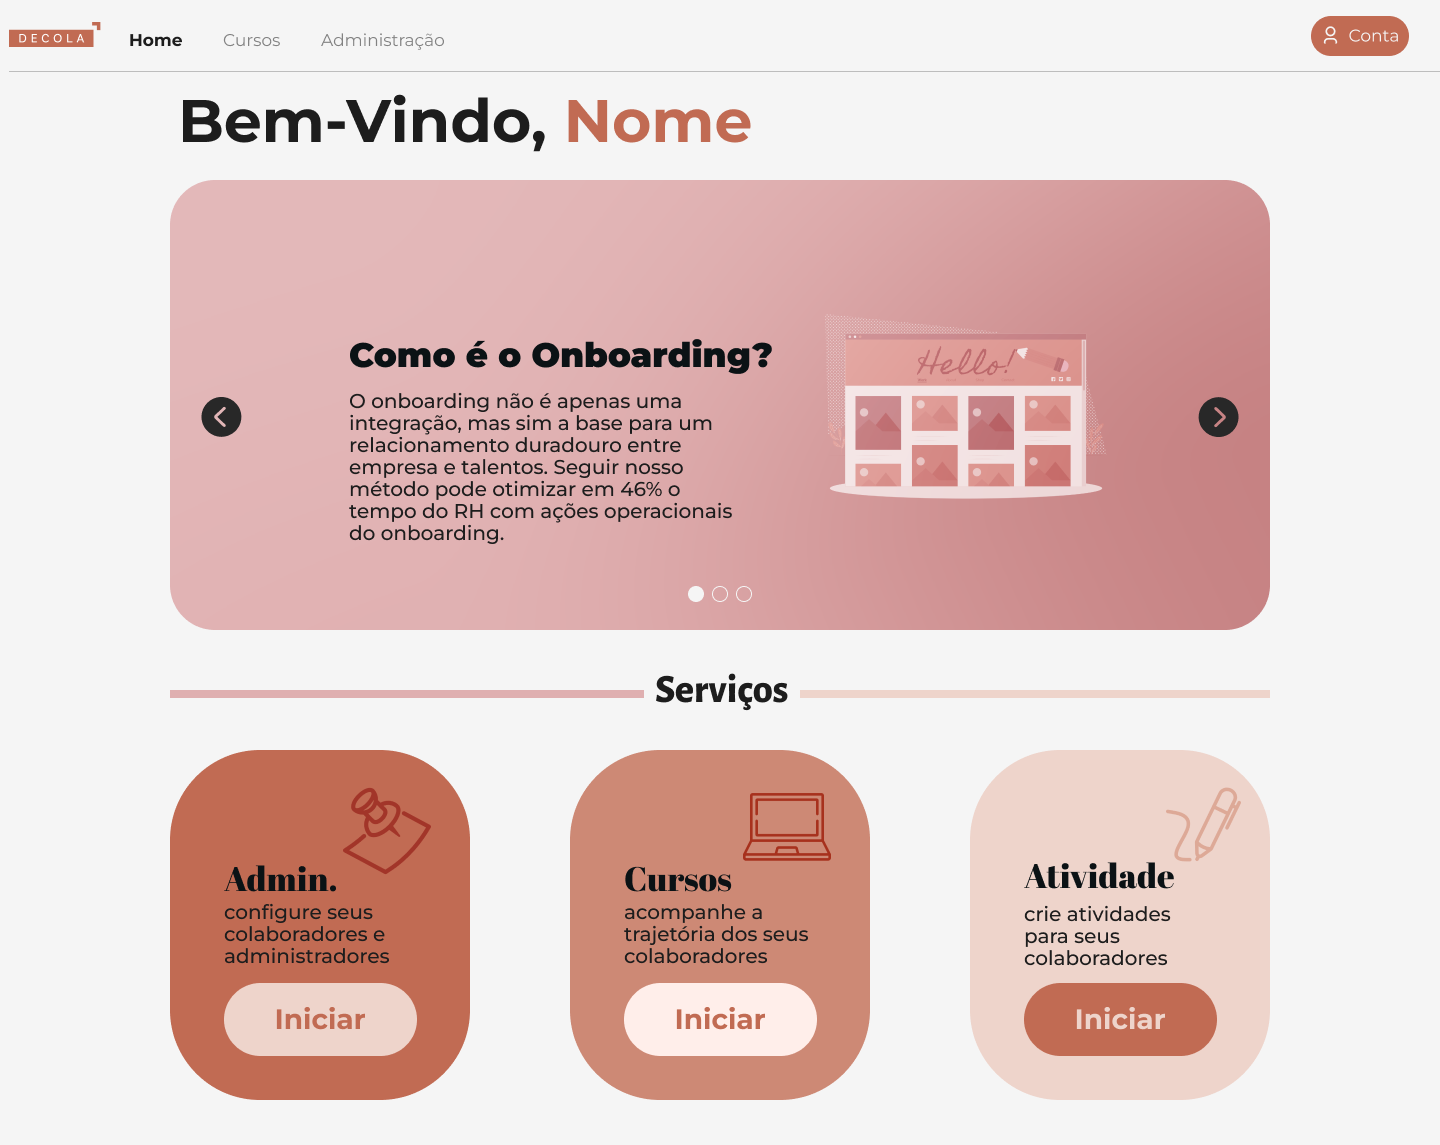
\includegraphics[width=1\linewidth]{conteudo//2 - ages I//conteudo//figures/mockup-decola-rh-inicial.png}
        Fonte: Wiki do Projeto
        \label{fig:rh-inicial-mockup-decola}
\end{figure}

    \begin{figure}[H]
        \centering
        \small
        \caption{Mockup Tela Inicial do RH - Decola}
        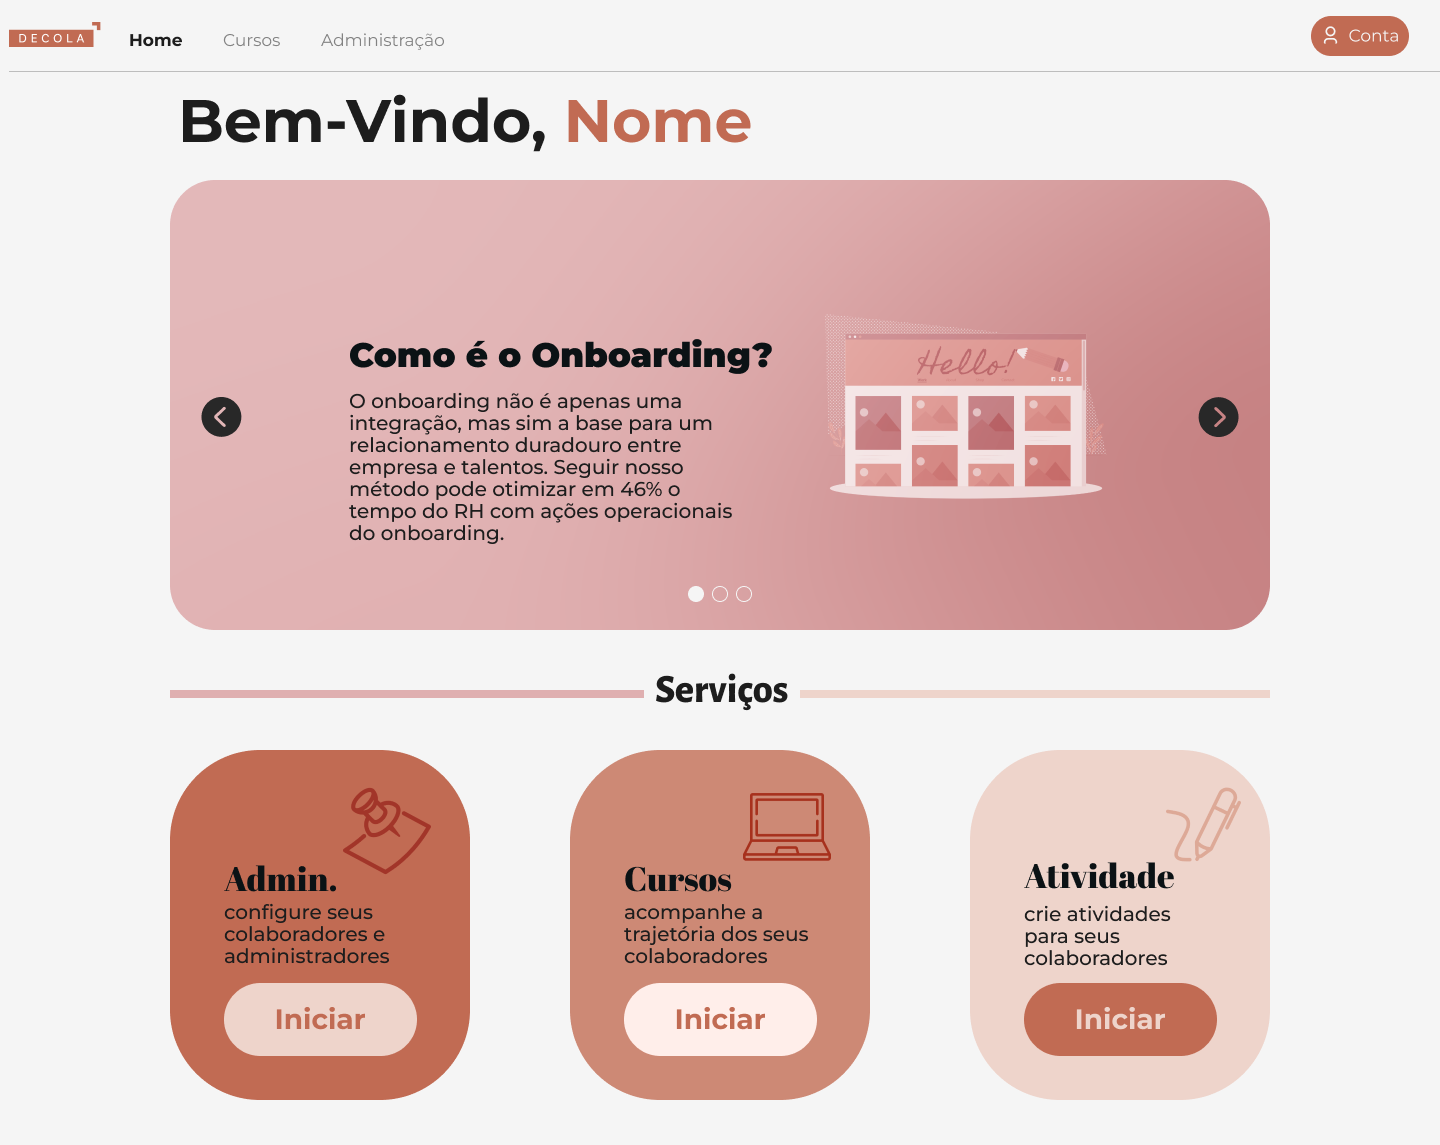
\includegraphics[width=1\linewidth]{conteudo//2 - ages I//conteudo//figures/mockup-decola-rh-inicial.png}
        Fonte: Wiki do Projeto
        \label{fig:rh-inicial-mockup-decola}
\end{figure}

    \begin{figure}[H]
        \centering
        \small
        \caption{Mockup Tela Dashboard do Administrador - Decola}
        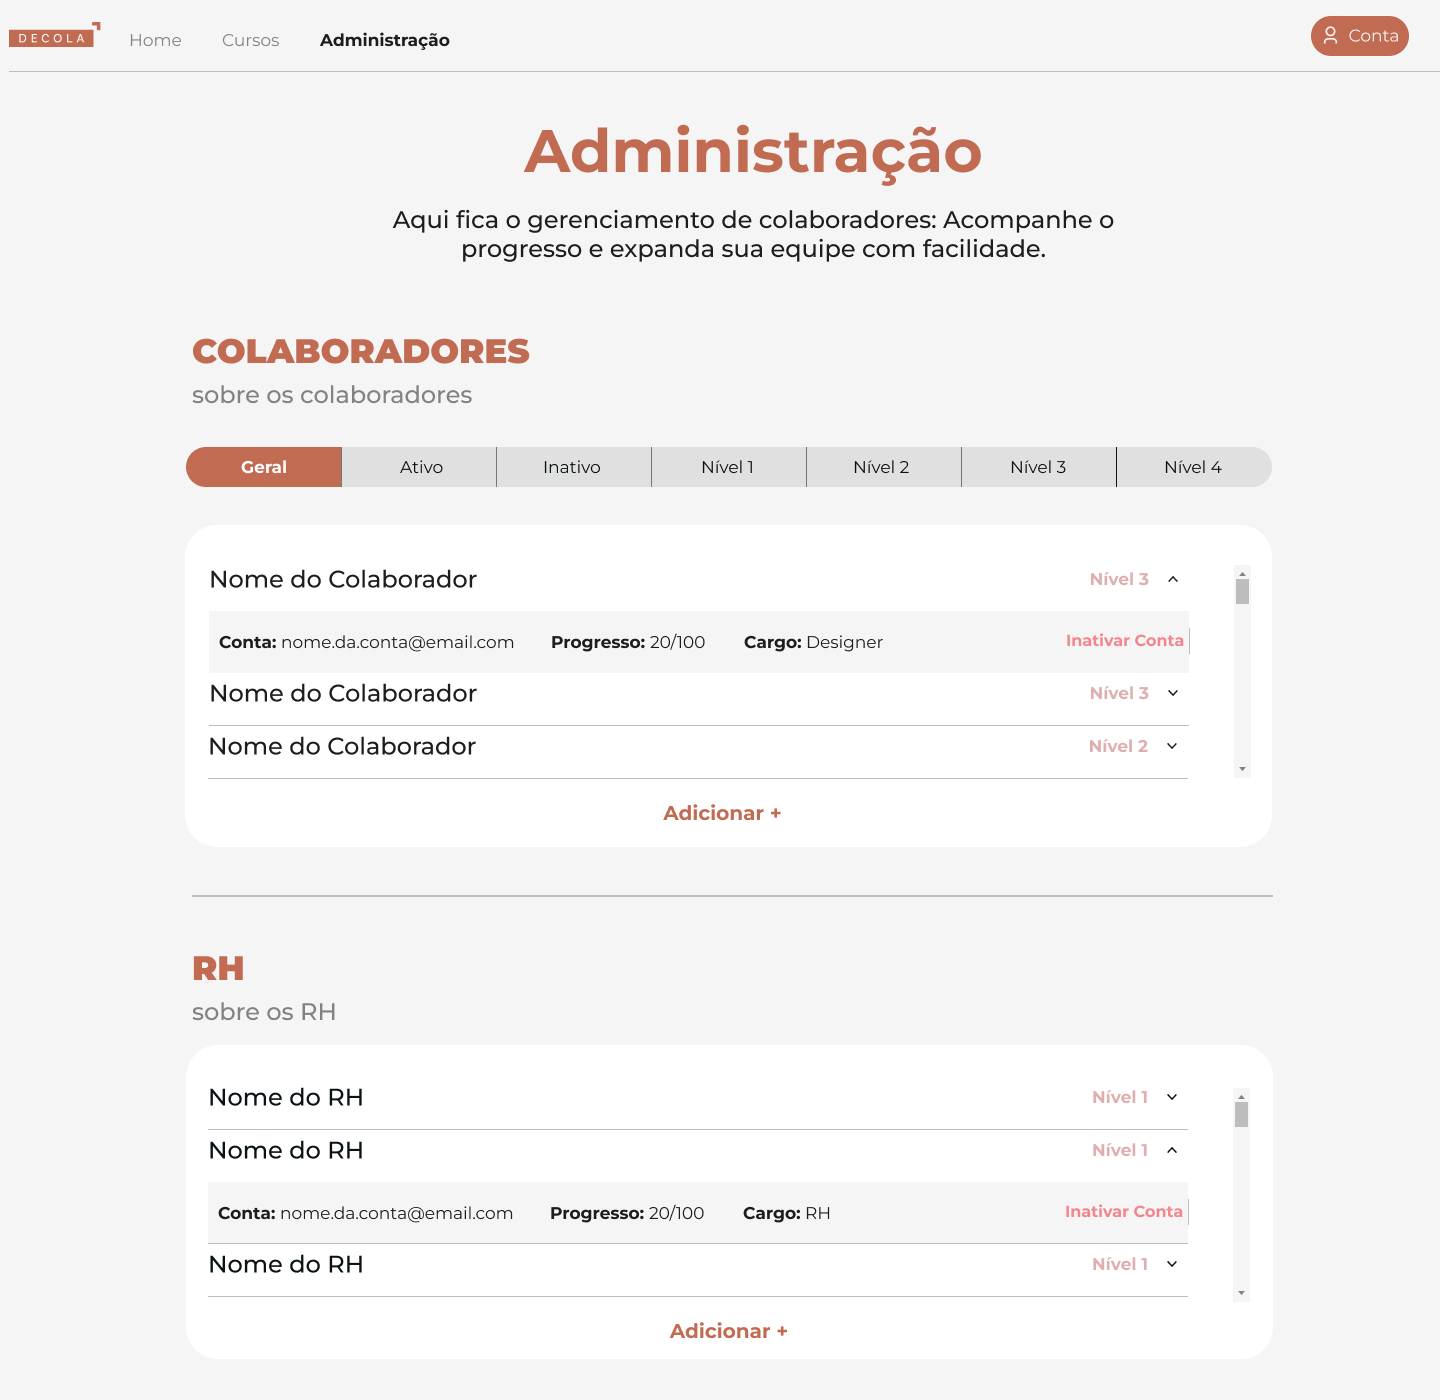
\includegraphics[width=1\linewidth]{conteudo//2 - ages I//conteudo//figures/mockup-decola-admin-dashboard.png}
        Fonte: Wiki do Projeto
        \label{fig:admin-dashboard-mockup-decola}
\end{figure}

    \begin{figure}[H]
        \centering
        \small
        \caption{Mockup Tela de Áreas do RH - Decola}
        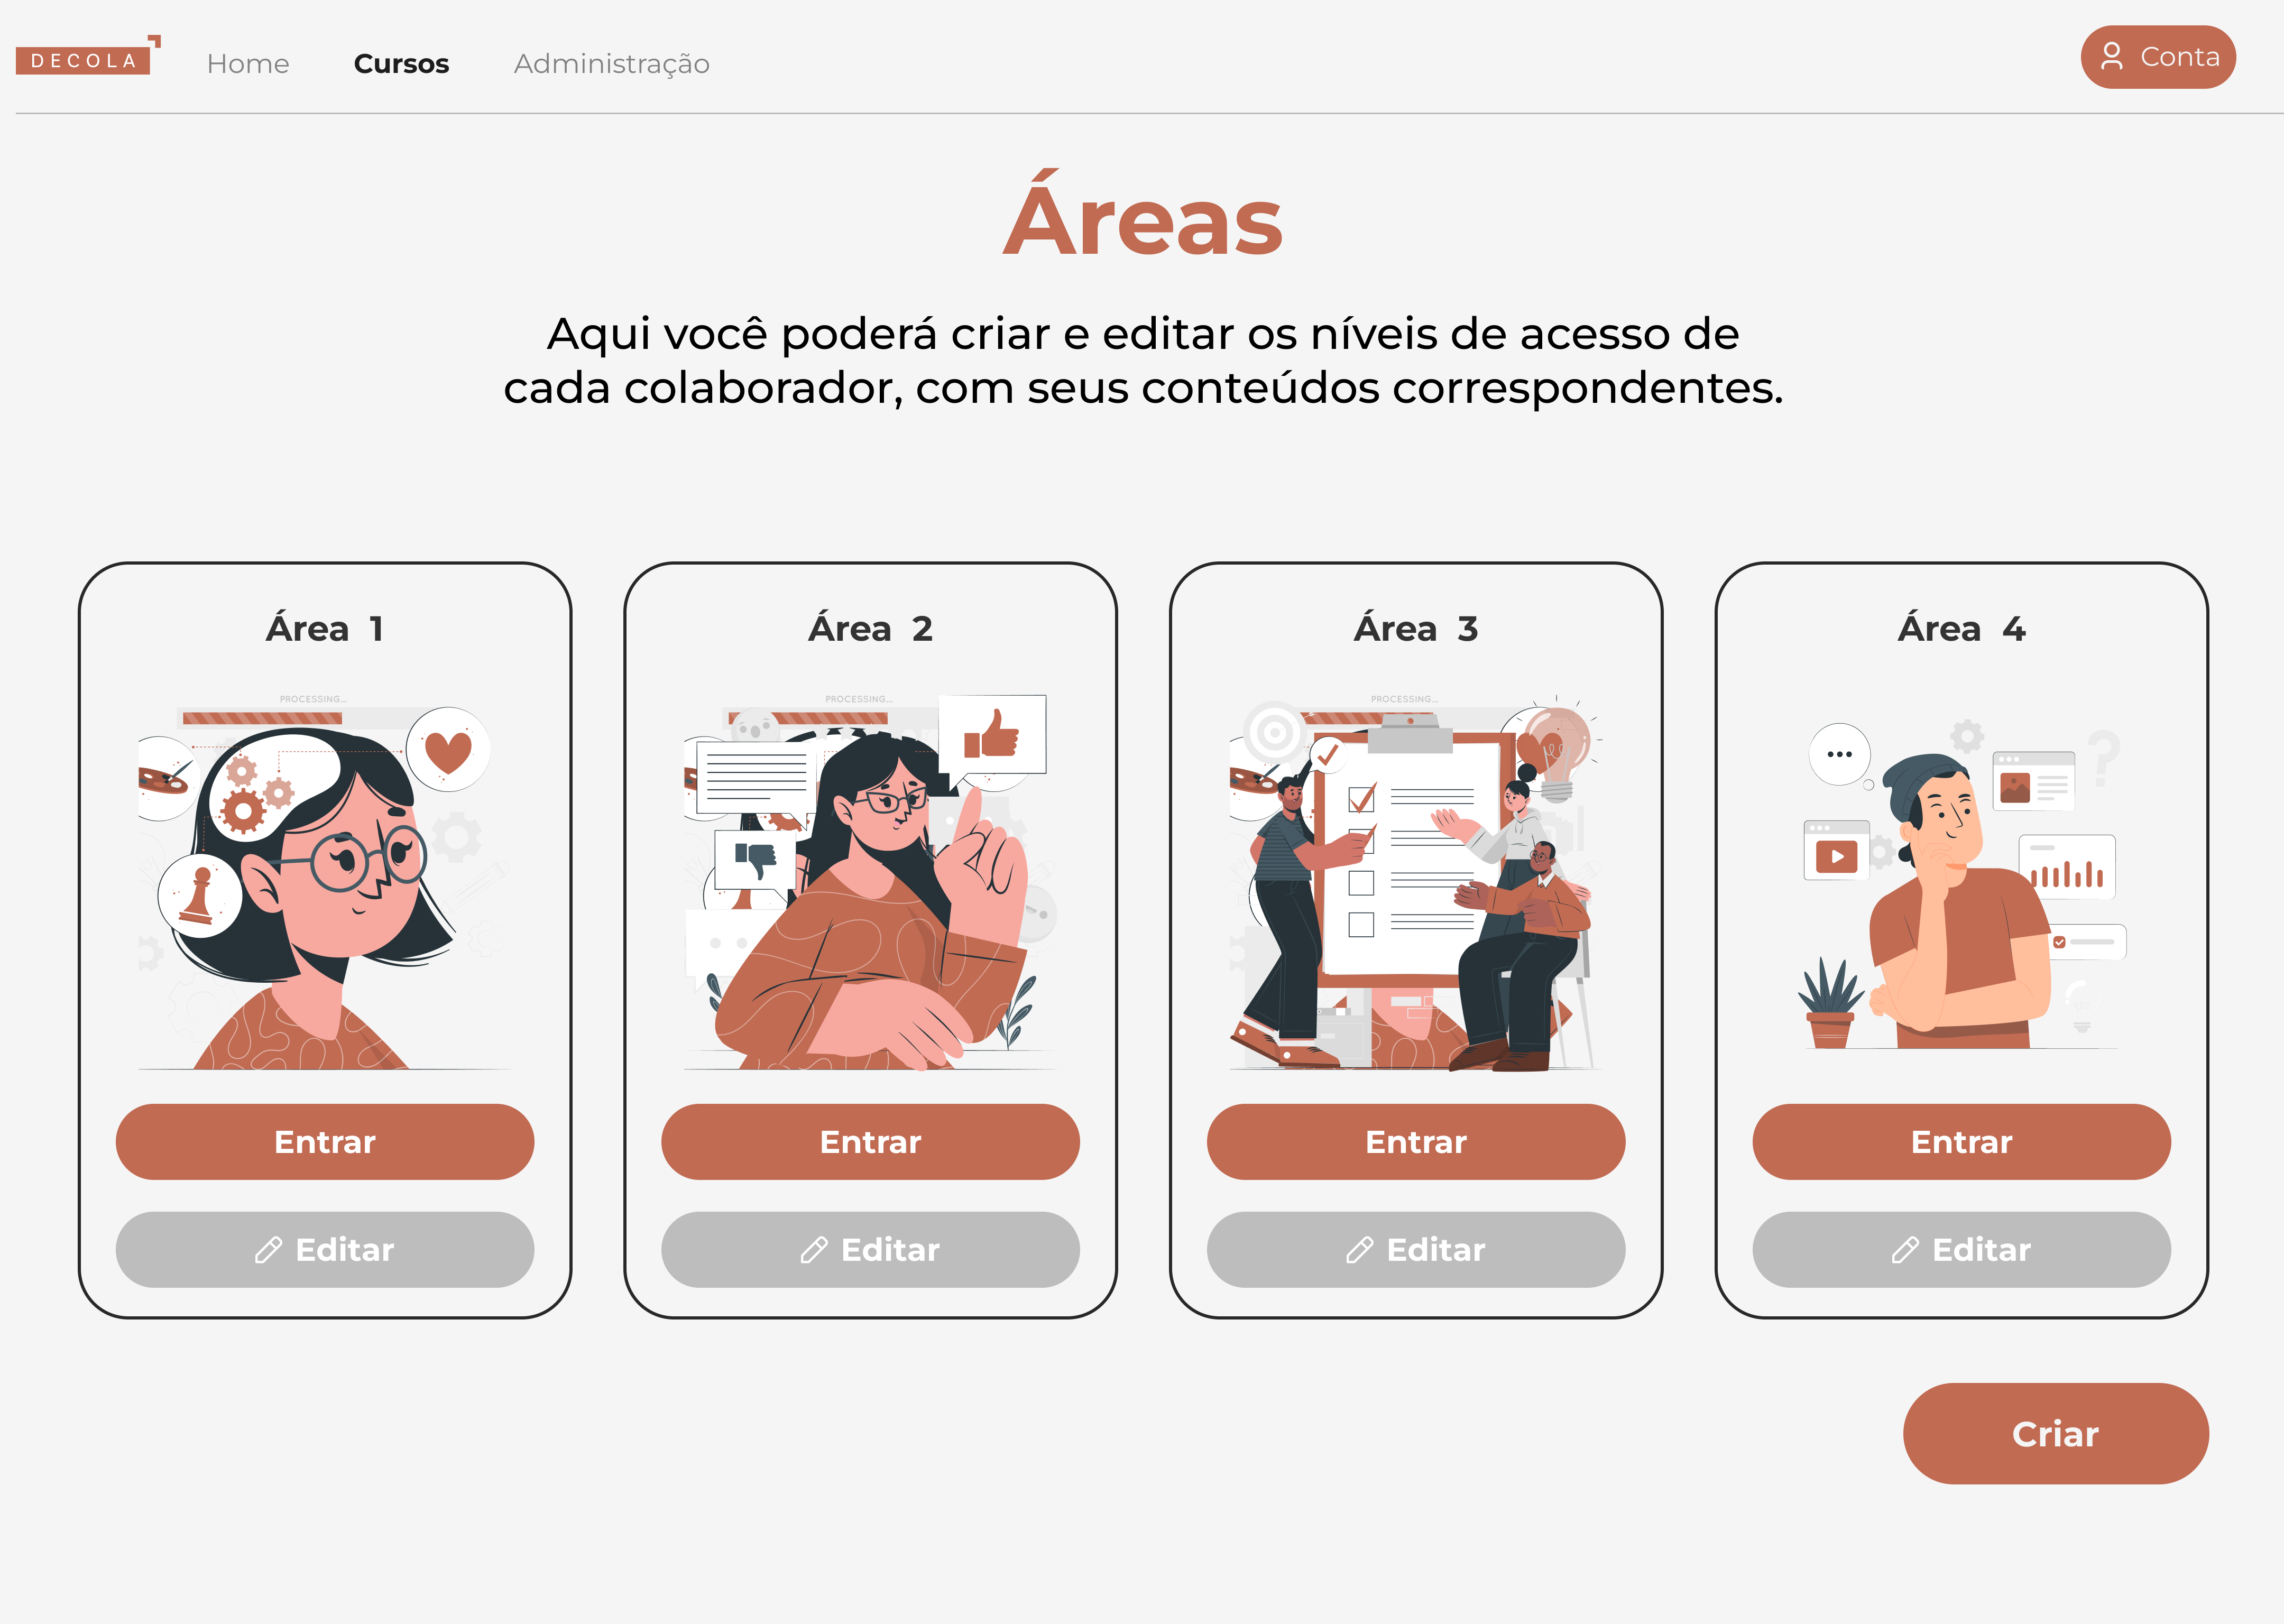
\includegraphics[width=1\linewidth]{conteudo//2 - ages I//conteudo//figures/mockup-decola-rh-areas.png}
        Fonte: Wiki do Projeto
        \label{fig:rh-areas-mockup-decola}
\end{figure}

    \begin{figure}[H]
        \centering
        \small
        \caption{Mockup Tela de Módulos do RH - Decola}
        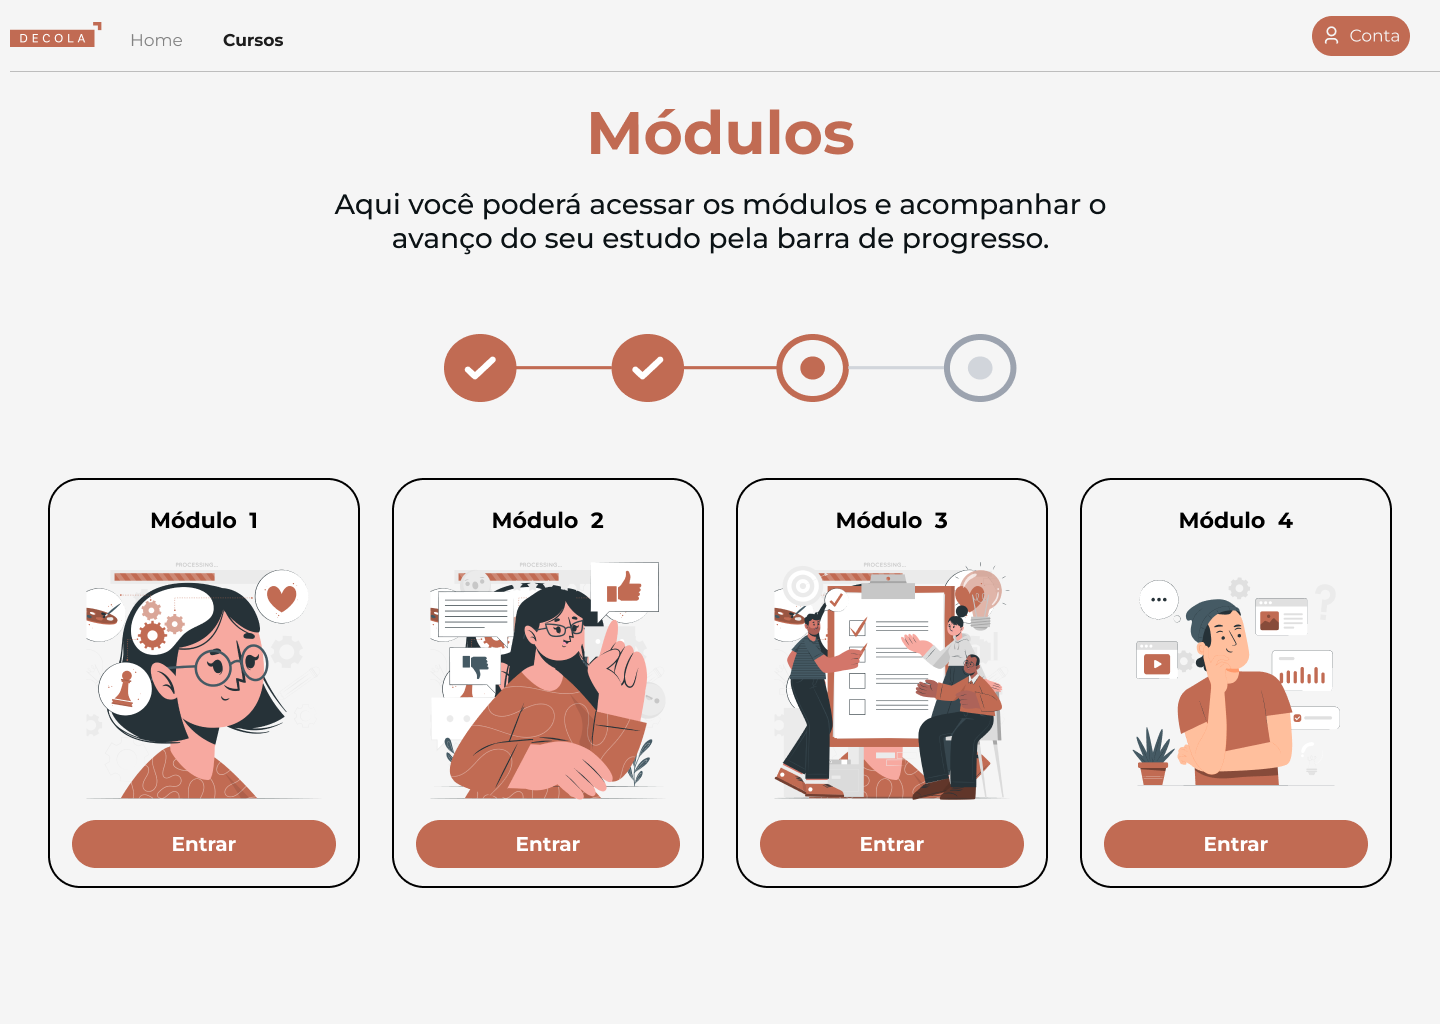
\includegraphics[width=1\linewidth]{conteudo//2 - ages I//conteudo//figures/mockup-decola-rh-modulos.png}
        Fonte: Wiki do Projeto
        \label{fig:rh-modulos-mockup-decola}
\end{figure}

    \begin{figure}[H]
        \centering
        \small
        \caption{Mockup Perguntas de Múltipla Escolha do RH - Decola}
        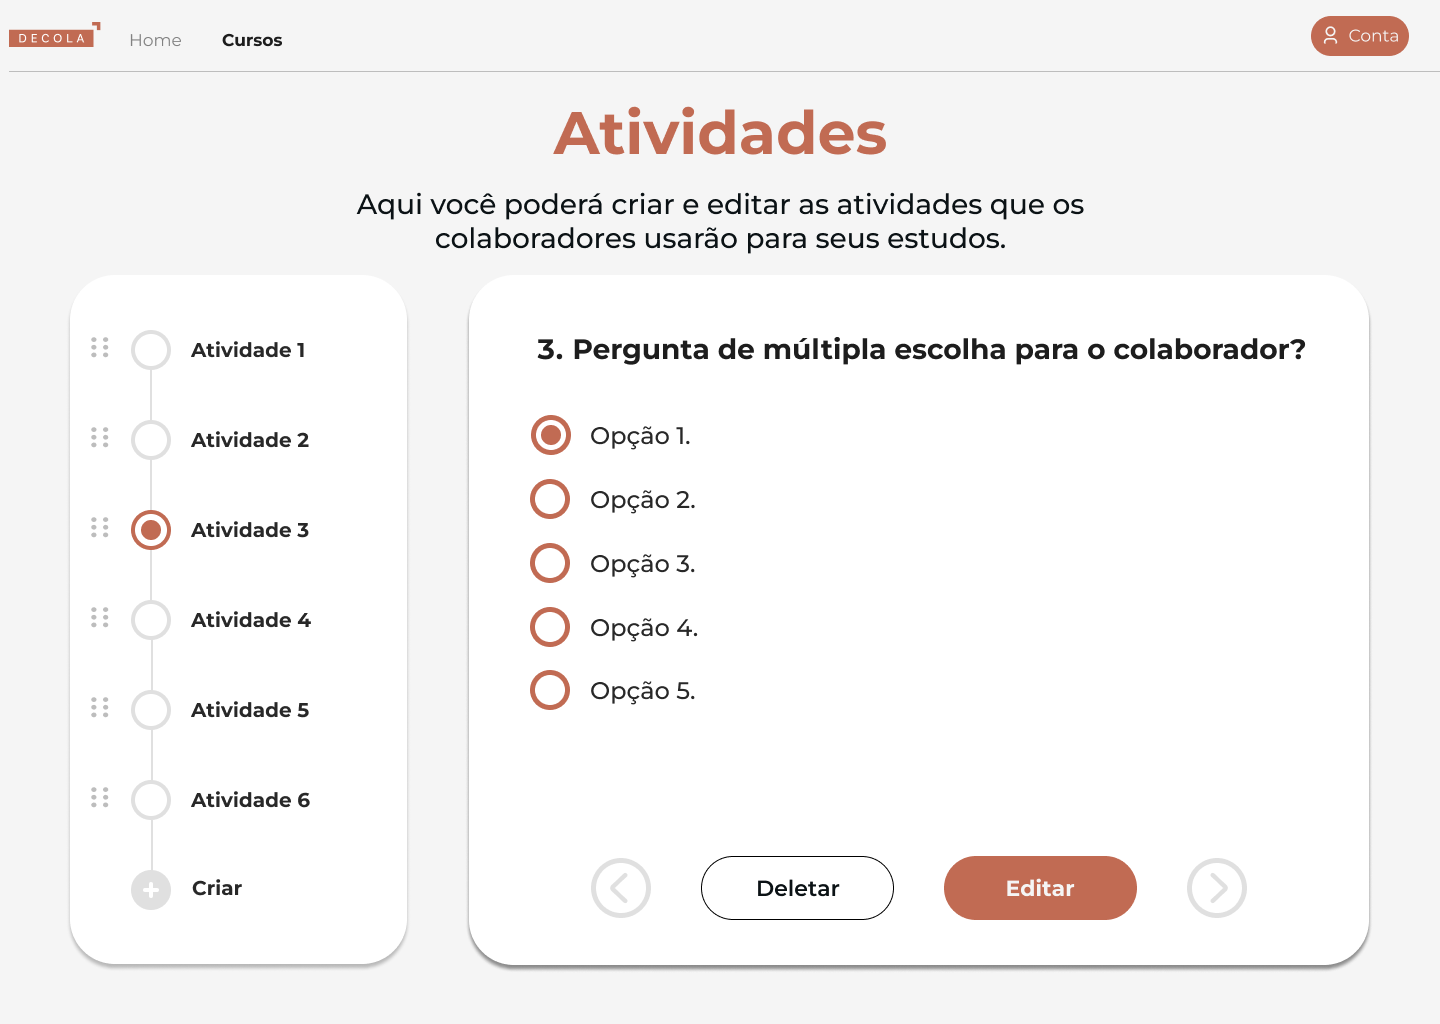
\includegraphics[width=1\linewidth]{conteudo//2 - ages I//conteudo//figures/mockup-decola-rh-single-choice.png}
        Fonte: Wiki do Projeto
        \label{fig:rh-single-choice-mockup-decola}
\end{figure}

    \begin{figure}[H]
        \centering
        \small
        \caption{Mockup Perguntas de Checkbox do RH - Decola}
        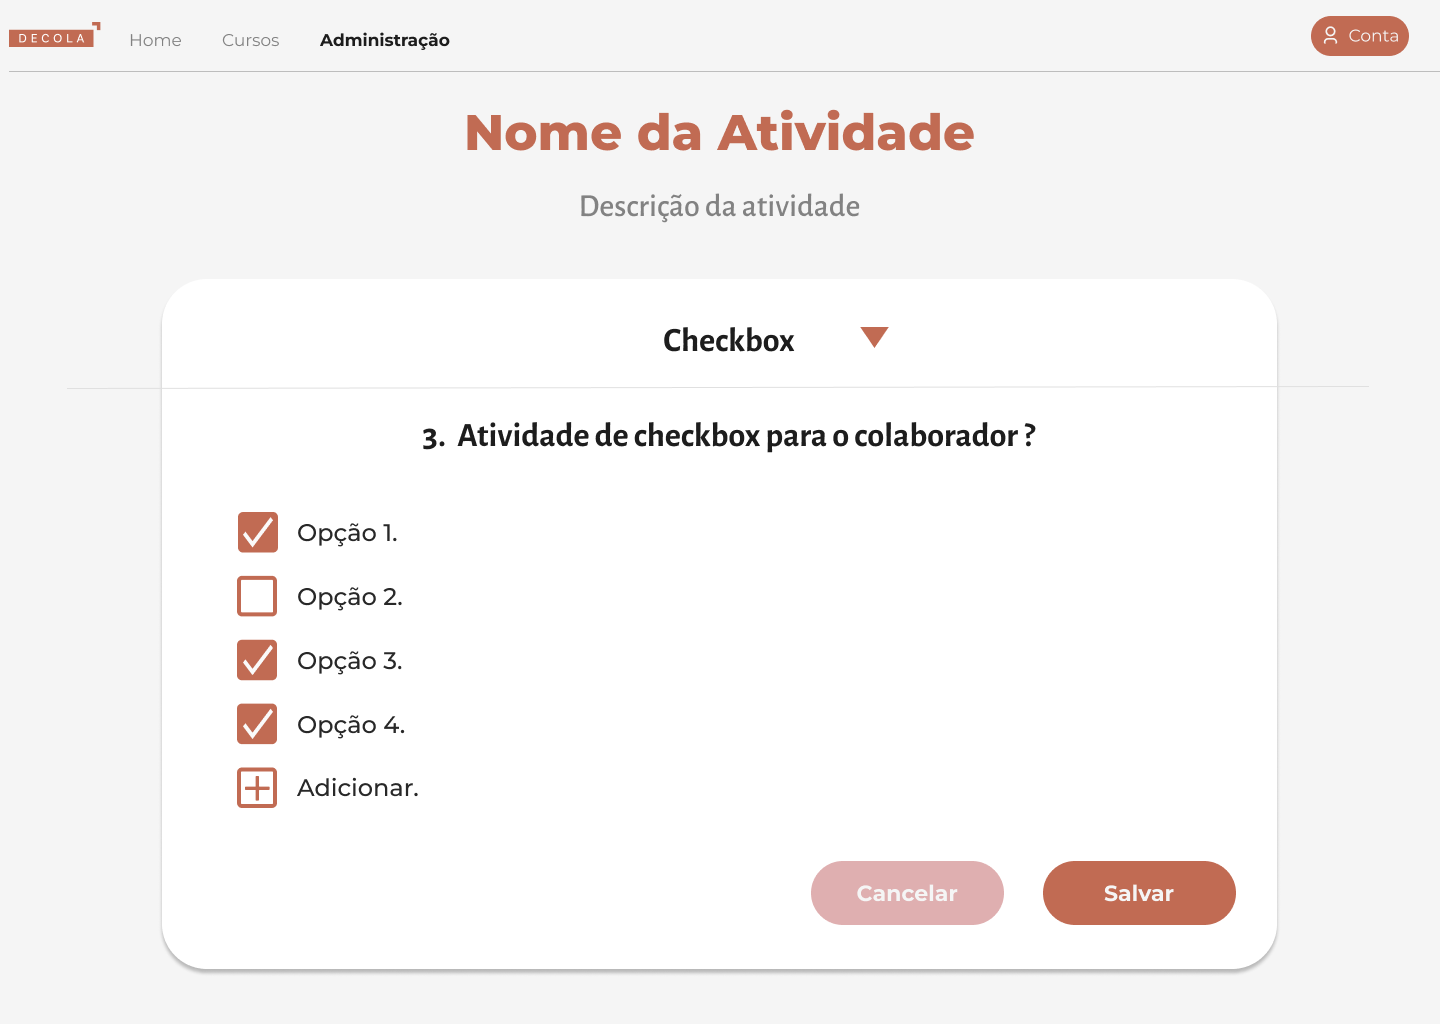
\includegraphics[width=1\linewidth]{conteudo//2 - ages I//conteudo//figures/mockup-decola-rh-checkbox.png}
        Fonte: Wiki do Projeto
        \label{fig:rh-checkbox-mockup-decola}
\end{figure}


\subsection{Tecnologias Utilizadas}
  Para o trabalhar com o back-end, foram selecionadas a linguem Python e o framework FastAPI. Python por ser mais conhecida pelos nossos AGES III ela foi escolhida além dela possuir um suporte para ser possível a implementação de inteligência artificial no projeto.
  
O front-end decidiu utilizar Expo a React Native, já que pelo fato que Expo é uma plataforma de código aberto e conjunto de ferramentas construída sobre o React Native, que por sua vez é um framework de desenvolvimento de aplicativos móveis, o que facilitaria ao longo do projeto.
Para o banco de dados foi utilizado o PostgreSQL já que estaríamos trabalhando com poucas tabelas e dessa forma tornando a escolha dele como modelo e provedor mais efetiva.

Para nos auxiliar na criação, escolha, e acompanhamento das  tarefas, foi definido o Azure DevOps ao invés do Trello que é uma escolha normal para a definição de tarefas.
  
  As tecnologias citadas deverão ter referências bibliográficas.
